\documentclass[journal]{IEEEtran}
%
% *** GRAPHICS RELATED PACKAGES ***
%
\ifCLASSINFOpdf
  \usepackage[pdftex]{graphicx}
  % declare the path(s) where your graphic files are
  % \graphicspath{{../pdf/}{../jpeg/}}
  % and their extensions so you won't have to specify these with
  % every instance of \includegraphics
  % \DeclareGraphicsExtensions{.pdf,.jpeg,.png}
\else
  % or other class option (dvipsone, dvipdf, if not using dvips). graphicx
  % will default to the driver specified in the system graphics.cfg if no
  % driver is specified.
  \usepackage[dvips]{graphicx}
  % declare the path(s) where your graphic files are
  % \graphicspath{{../eps/}}
  % and their extensions so you won't have to specify these with
  % every instance of \includegraphics
  % \DeclareGraphicsExtensions{.eps}
\fi
\ifCLASSOPTIONcompsoc
  \usepackage[caption=false,font=normalsize,labelfont=sf,textfont=sf]{subfig}
\else
  \usepackage[caption=false,font=footnotesize]{subfig}
\fi
%
\usepackage{amsmath,amssymb}
\usepackage{color}
\newcommand{\red}[1]{\textcolor{red}{#1}}
\usepackage{ulem} % \sout{}
%
\begin{document}
%
% paper title
\title{Far-sidelobe Measurements of LiteBIRD \\ Low Frequency Telescope Scaled Model}
%%%
%
% author names and IEEE memberships
% note positions of commas and nonbreaking spaces ( ~ ) LaTeX will not break
% a structure at a ~ so this keeps an author's name from being broken across
% two lines.
% use \thanks{} to gain access to the first footnote area
% a separate \thanks must be used for each paragraph as LaTeX2e's \thanks
% was not built to handle multiple paragraphs
%
\author{Hayato~Takakura, Yutaro~Sekimoto, Junji~Inatani, Shingo~Kashima, Hiroaki~Imada, Takashi~Hasebe, Toru~Kaga, Yoichi~Takeda, and~Norio~Okada%~\IEEEmembership{Life~Fellow,~IEEE}% <-this % stops a space
\thanks{H. Takakura is with Department of Astronomy, School of Science, University of Tokyo, Tokyo Japan e-mail: takakura@astro.isas.jaxa.jp}% <-this % stops a space
\thanks{H. Takakura, Y. Sekimoto, J. Inatani, T. Hasebe, T. Kaga, Y. Takeda and N. Okada are with Institute of Space and Astronautical Science (ISAS), Japan Aerospace Exploration Agency (JAXA).}% <-this % stops a space
\thanks{S. Kashima and N. Okada are with National Astronomical Observatory of Japan.}% <-this % stops a space
\thanks{H. Imada are with Laboratoire de l'Accélérateur Linéaire, Université Paris-Sud, CNRS/IN2P3, Université Paris-Saclay.}% <-this % stops a space
\thanks{Manuscript received XXXXX; revised XXXXX.}}
%%%
%
% The paper headers
\markboth{IEEE Transactions on Terahertz Science and Technology,~Vol.~XX, No.~X, November~2019}%
{Shell \MakeLowercase{\textit{et al.}}: Bare Demo of IEEEtran.cls for IEEE Journals}
% The only time the second header will appear is for the odd numbered pages
% after the title page when using the twoside option.
% 
% *** Note that you probably will NOT want to include the author's ***
% *** name in the headers of peer review papers.                   ***
% You can use \ifCLASSOPTIONpeerreview for conditional compilation here if
% you desire.
%%%
%
% If you want to put a publisher's ID mark on the page you can do it like
% this:
%\IEEEpubid{0000--0000/00\$00.00~\copyright~2015 IEEE}
% Remember, if you use this you must call \IEEEpubidadjcol in the second
% column for its text to clear the IEEEpubid mark.
%
% use for special paper notices
%\IEEEspecialpapernotice{(Invited Paper)}
%
% make the title area
\maketitle
%
% As a general rule, do not put math, special symbols or citations
% in the abstract or keywords.
\begin{abstract}
The abstract goes here.
\end{abstract}
%
% Note that keywords are not normally used for peerreview papers.
\begin{IEEEkeywords}
XXX, YYY, ZZZ.
\end{IEEEkeywords}
%
% For peer review papers, you can put extra information on the cover
% page as needed:
% \ifCLASSOPTIONpeerreview
% \begin{center} \bfseries EDICS Category: 3-BBND \end{center}
% \fi
%
% For peerreview papers, this IEEEtran command inserts a page break and
% creates the second title. It will be ignored for other modes.
\IEEEpeerreviewmaketitle
%
%
%
\section{Introduction}
% You must have at least 2 lines in the paragraph with the drop letter
% (should never be an issue)
%
% The very first letter is a 2 line initial drop letter followed
% by the rest of the first word in caps.
% 
% form to use if the first word consists of a single letter:
% \IEEEPARstart{A}{demo} file is ....
% 
% form to use if you need the single drop letter followed by
% normal text (unknown if ever used by the IEEE):
% \IEEEPARstart{A}{}demo file is ....
% 
% Some journals put the first two words in caps:
% \IEEEPARstart{T}{his demo} file is ....
% 
% Here we have the typical use of a "T" for an initial drop letter
% and "HIS" in caps to complete the first word.
%
\IEEEPARstart{I}{nflation} theory describes that the universe began with a drastic expansion of the space, causing primordial gravitational waves\cite{Guth1981}. One of the most promising ways to investigate the universe at this era is precise observation of the polarization of Cosmic Microwave Background (CMB) \cite{Kamionkowski1997,Seljak1997}. It is predicted that the primordial gravitational waves have created so-called B-mode polarization patterns at angular scale of several degrees with intensity of less than hundreds nano-kelvins~\red{[cite]}. 
\par
LiteBIRD is a Strategic Large Mission of Japan Aerospace Exploration Agency to investigate polarization of CMB from space~\cite{Hazumi2012, Sekimoto2018}. It is planned to be launched in $\sim$2027 and aims to detect B-mode polarization at the level of $\delta r > 0.001$, where $r$ is the scalar tensor ratio. 
\par
Space programs of CMB B-mode polarization observations after the Planck satellite \cite{Planck2018} require broader frequency bands, wider field of view (FoV) to detect a small polarization signals of the large scale. Far-sidelobes cause contamination of the CMB signals from strong radiations from outside of the pointing direction, especially from the galactic plane. It is is one of the most challenging issues for wide FoV telescopes to suppress the far-sidelobes.  
A previous study~\cite{Tran2010} requires a level of $\sim -60~\mathrm{dB}$.
Since allocated volume and mass of space telescopes are limited by the cost cap, lower sidelobe level should be carefully designed for small aperture telescope with large FoV.
 
\par
Low Frequency Telescope (LFT), one of the telescopes equipped with LiteBIRD, observes 34--161~GHz for CMB signals and synchrotron radiation foreground. The aperture diameter is 400~mm and the field of view is $20^\circ \times 10^\circ$. To reduce the thermal noises, the whole telescope is operated below 5~K.
%\par
%According to the former studies on the systematic errors~\red{[cite]}, 
Requirements on LFT are far-sidelobes knowledge at the level of -56~dB
and cross-polarization of less than -20~dB \cite{Sekimoto2018}. The optical design of LFT has been studied so as to satisfy these requirements \cite{Kashima2018,Imada2018}.
LFT has adopted a cross-Dragone optical system~\cite{Dragone1978} with the crossing angle of the optical axes of 90 degrees and F\# of 3.0.
\par
This study aims to examine the optical performance of LFT, and especially focuses on far-sidelobe measurement to confirm that the far-sidelobes can be calibrated with the accuracy of -56 dB. In the past CMB experiments, the far-sidelobes were measured with far-field measurement \red{[cite BICEP]} or compact range measurement \red{[cite Planck]}. Since these measurement methods require a huge facility, they are not suitable for the studies of telescopes under development. We have therefore adopted near-field beam measurement method \cite{Yaghjian1984}, which enables to make the measurement facility compact by calculating the beam pattern of an antenna from amplitude and phase distributions near the aperture, instead of directly measuring the far field pattern. This method is widely used during the development of other radio telescopes such as Atacama Large Millimeter/submillimeter Array~\cite{Naruse2009} \red{+ Alvaro's paper}. 
\par
We have developed a 1/4-scaled model of LFT for beam pattern measurements of LFT, so that minor changes of the optical design can be easily examined. Not only LFT itself but also the measurement wavelength are scaled to 1/4 size to know the beam pattern.
%
% (End of Introduction)
%
\section{LFT 1/4-scaled model}
%
\subsection{Design and Fabrication}
%
\par
We have built a 1/4-scaled model of LFT based on an optical design with F/\#3.0 and the cross angle of 90 degree. 
%It was built as an assembly of three separated components, a frame and primary/secondary mirrors, each of which was machined from an aluminum block (A5052) using a 5-axis machining center (Makino D500) and a wire-electrical discharge machine (Mitsubishi Electric MV2400R). 
A frame and primary/secondary mirrors of the scaled LFT (Figure \ref{fig:cad-frame-mirrors}) has been designed and built at the machine shop of ISAS/JAXA.
The frame has been machined from an aluminum block (A5052) with a wire-electrical discharge machine (Mitsubishi Electric MV2400R).
The mirrors have been fabricated with a 5-axis machining center (Makino D500).
Its size and weight are $230 \times 250 \times 300 ~\mathrm{mm}$ and 7.6~kg respectively. To reduce multi-path reflections, ECCOSORB AN72 was attached on the frame and the edge of the mirrors.
\red{A front hood has been fabricated ...}
%
\begin{figure}
\centering
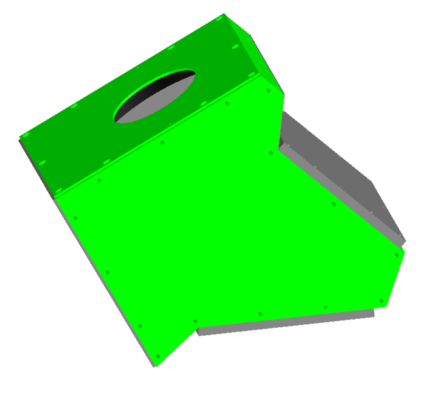
\includegraphics[width=0.6\linewidth]{Figures/cad1.pdf}
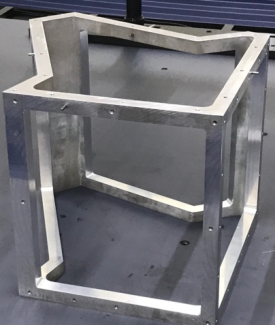
\includegraphics[width=0.6\linewidth]{Figures/frame.pdf}
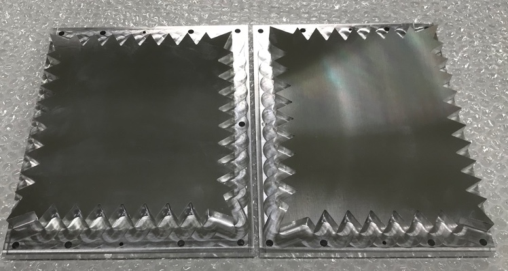
\includegraphics[width=0.6\linewidth]{Figures/mirrors.pdf}
\caption{(Top) a cad model of scaled model.\red{(pls provide captions of focal plane and aperture)} (middle) a frame. (bottom) a primary mirror and secondary mirror }
\label{fig:cad-frame-mirrors}
\end{figure}
\par
% \red{(Description of focal plane and wide field of view)}
The scaled LFT has a focal plane area of 100 mm $\times$ 50 mm to cover wide field of view 20 degree $\times$ 10 degree.  
Antenna patterns are measured at three positions of the focal plane as shown in Figure~\ref{fig:FeedPos}. For each position, the measurement was conducted for two orthogonal polarization directions, V-pol (vertical polarization) and H-pol (horizontal polarization).
%
%During the measurement, the conical horn antenna was placed at three positions on the focal plane, as shown in Figure~\ref{fig:FeedPos}. For each feed horn position, the measurement was conducted for two orthogonal polarization directions, V-pol (vertical polarization) and H-pol (horizontal polarization).
%
\subsection{Mechanical Errors}
%
We have studied the manufacturing tolerance using Synopsys Code V. \sout{This study \red{(reported at Annual Meeting of Astronomical Society of Japan 2019 Spring by Kashima-san)} shows that the manufacturing tolerance is limited by rotation tolerance of the polarization direction.} Based on this study, we have defined the manufacturing tolerance as 1~mm and 30~arcsec for the translational and rotational errors respectively, for both the primary and secondary mirrors (see Table \ref{tb:mech_err}).
\par
To check whether the 1/4-scaled LFT satisfies these requirement, the alignment accuracy and surface accuracy of the mirrors were measured by a 3-dimensional coordinate measuring machine (Mitsutoyo LEGEX 12128) with a contact probe. 100 points on the surface of each mirror were measured. As shown in Table \ref{tb:mech_err}, the translational and rotational errors were \red{$XX~\mathrm{\mu m}$} and \red{XX~arcsec} at the maximum respectively. The surface accuracy was \red{$XX~\mathrm{\mu m}$} rms for the primary mirror and \red{$XX~\mathrm{\mu m}$} rms for the secondary mirror. These numbers satisfy the defined tolerance.
%
\begin{table}[!t]
% increase table row spacing, adjust to taste
\renewcommand{\arraystretch}{1.3}
% if using array.sty, it might be a good idea to tweak the value of
% \extrarowheight as needed to properly center the text within the cells
\caption{Mechanical Errors of the Scaled Model}
\label{tb:mech_err}
\centering
% Some packages, such as MDW tools, offer better commands for making tables
% than the plain LaTeX2e tabular which is used here.
\begin{tabular}{|c|ccc|ccc|}
\hline
Mirror & \multicolumn{3}{|c}{Translational Error /mm} & \multicolumn{3}{|c|}{Rotational Error /arcsec} \\
 & $x$ & $y$ & $z$ & $\phi_x$ & $\phi_y$ & $\phi_z$ \\
\hline
Primary & XX & YY & ZZ & XX & YY & ZZ \\
(Tolerance) & XX & YY & ZZ & XX & YY & ZZ \\
\hline
Secondary & XX & YY & ZZ & XX & YY & ZZ \\
(Tolerance) & XX & YY & ZZ & XX & YY & ZZ \\
\hline
\end{tabular}
\end{table}
%
% (End of 1/4-scaled model)
%
\section{Measurement system}
%
\subsection{Near-field Beam Measurement System}
\par
A near-field beam measurement system based on a vector network analyzer (VNA) has been developed to characterize the scaled LFT (Figure~\ref{fig:MeasSys}). 
The VNA consists of a microwave part (Keysight N5222B) and WR5.1 frequency extenders (140 - 220 GHz) of transmitter and receiver modules (Virginia Diodes Inc.).
A probe horn with the receiver module measures both the amplitude and phase distributions near the aperture with a $XY\Phi$ scanner. It is possible to rotate the polarization direction of the probe horn (open-ended waveguide). 
A horn with the transmitter module is placed at an arbitrary position on the focal plane with a $XYZ$ stage.
These arrangement is a time-reverse configuration of a real CMB observation.
\red{Pls add specifications (scan range, flattness, ...) of these scanners.} 
A dedicated Python script has been developed to control the system using PyVISA package\footnote{https://pyvisa.readthedocs.io/}.
\par
Since the antenna has been scaled in 1/4 dimension, the measurement wavelength has been accordingly scaled. We have therefore chosen the measurement frequencies as 140, 160, 180, 200 and 220~GHz, which correspond to 35--55~GHz of a full-scale LFT. 
This frequency range roughly corresponds to the lowest frequencies of LFT bands, named LF1 (34--99~GHz) with a lens diameter of 24 mm and \red{MF1 (60--137~GHz)} with a lens diameter of 16 mm, at which it is expected to show larger far-sidelobes due to diffraction.  
\par
The amplitude and phase are probed every 0.5~mm with a WR5.1 open waveguide (hereafter referred as a probe horn) in the rectangular area of $180 \times 180~\mathrm{mm}$ around the aperture. The probe horn with an aperture of \red{1.x mm $\times$ 0.y mm} has the tapered edge to reduce the return loss at the aperture. The sampling spacing was determined so as to satisfy the Nyquist condition. \red{The measurement area is optimized in advance to get a far-field beam pattern with errors of less than -70~dB level. ?} 
Current scan takes around 30 hours to obtain the 5-frequency beam patterns for each feed horn position and one polarization angle. 
It can be reduced by optimizing the sequence of the data acquisition.
%
\begin{figure}[!t]
\centering
\includegraphics[width=0.9\linewidth]{Figures/MeasSys.pdf}
\caption{A 1/4-scaled model of LFT and its near-field beam measurement system. A conical horn with a transmitter of a VNA scans the focal plane of LFT with a XYZ stage. A probe horn with a receiver measures the amplitude and phase distributions near the aperture with a XY$\Phi$ stage. 
% The system is controlled by a dedicated Python script.
}
\label{fig:MeasSys}
\end{figure}
%
%
\subsection{Feed Horn}
\par
LiteBIRD LFT focal plane has TES bolometer arrays with sinuous antennas and lenslets, \sout{which have been currently under development} \cite{Suzuki2018}. 
The beam patterns have been characterized as a main lobe has a shape of Gaussian beam \cite{Edwards2012}. 
The optical design of LFT is assumed with Gaussian beam with beam waist radius of 9.412~mm for the 34 - 87 GHz band with lens-let diameter of 24 mm and 8.727~mm for the 60 - 137 GHz band with lens-let diameter of 16 mm.
\par 
A smoothed-wall conical horn has been used as a feed of the 1/4 LFT, whose aperture diameter and length are 10.4~mm and 20~mm, respectively. Its beam pattern has been measured in advance using the near-field beam scanner. The results are shown in Figure~\ref{fig:Feedhorn}. The measured beam width of the conical horn was $\lesssim 10\%$ larger at 180~GHz and $\lesssim 15\%$ larger at 140 and 220~GHz than that of the Gaussian-approximated beam patterns of the sinuous antenna.

\begin{figure}[!t]
\centering
\subfloat[Beam patterns of a conical horn at 180~GHz \red{Pls provide higher resolution of FFT}]{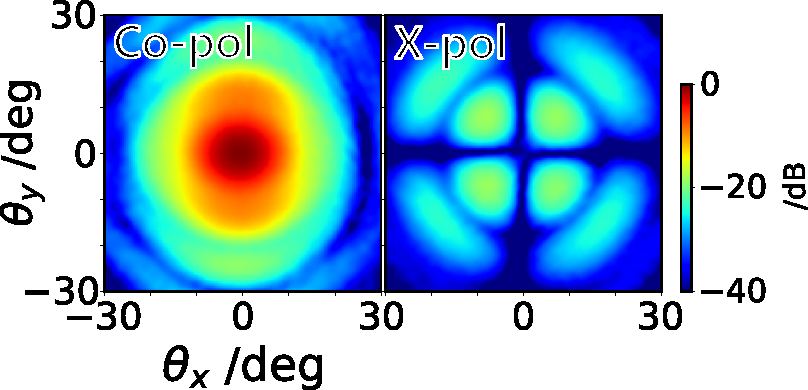
\includegraphics[width=0.9\linewidth]{Figures/FeedHornPattern.pdf}%
\label{fig:FeedHornPattern}}
\hfil
\subfloat[Comparison with \sout{LF1/LF2} Gaussian beam]{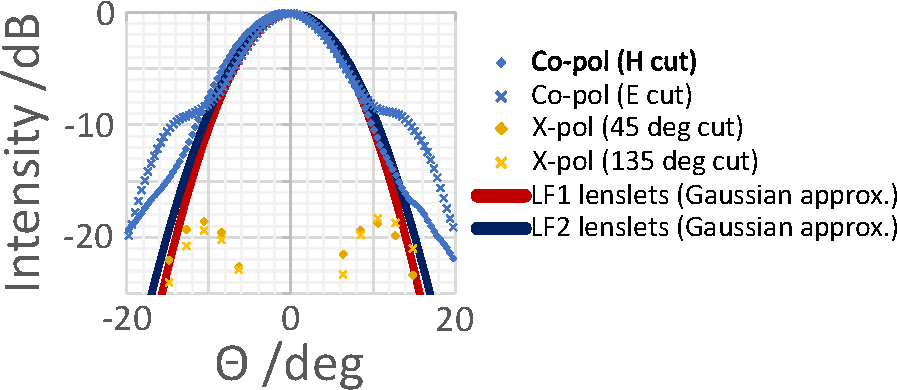
\includegraphics[width=0.9\linewidth]{Figures/FeedHorn_vs_Lenslet.pdf}%
\label{fig:FeedHorn_vs_Lenslet}}
\caption{%
\protect\subref{fig:FeedHornPattern} Beam patterns of a conical horn used as the feed, measured at 180~GHz (corresponding to 45~GHz of the full-scale model). Co-pol and X-pol stand for co-polarization and cross-polarization respectively, and the E-plane is parallel to the $\theta_y$ axis. The maximum cross-polarization level is -17~dB.
\protect\subref{fig:FeedHorn_vs_Lenslet} The dots show the $\theta_y = 0$ cut ($\phi = 0$; H cut) and $\theta_x = 0$ cut ($\phi = 90^\circ$; E cut) of the measured co-polarization beam patterns of the conical horn at 180~GHz, as well as $\phi=45^\circ$ and $\phi=135^\circ$ cuts of the measured cross-polarization patterns. The solid lines show the Gaussian beams, which are an approximation to the beam patterns of the sinuous antennas and lenslets. \red{LF1 and LF2 (No definition)} are two lowest frequency bands of LFT.
}
\label{fig:Feedhorn}
\end{figure}
%
\begin{figure}[!t]
\centering
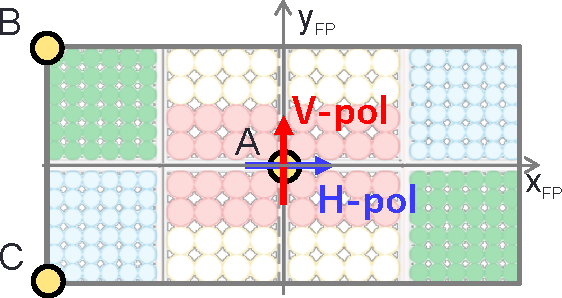
\includegraphics[width=0.8\linewidth]{Figures/FeedPos.pdf}
\caption{A schematic of the focal plane and feed positions. The colored circles show the positions and sizes of the lenslets. A, B and C show the positions where the feed is placed during the measurement, which are ($x_\mathrm{FP}$ /mm, $y_\mathrm{FP}$ /mm) = (0, 0), (23.25, -48.75), (-23.25, 48.75) on the focal plane. H-pol and V-pol are two orthogonal polarization directions of the feed horn.}
\label{fig:FeedPos}
\end{figure}
%
% (End of Measurement System)
%
\section{Data Processing}
%
\subsection{Coordinate}
\par
We have adopted right-handed coordinates system defined as follows: $z$ axis corresponds to the optical axis of LFT, whose direction is from the aperture to the focal plane. $x_\mathrm{FP}$ and $y_\mathrm{FP}$ are defined on the focal plane as shown in Figure~\ref{fig:FeedPos} . $x$ and $y$ are defined on the aperture plane such that $x$ axis is parallel to $x_\mathrm{FP}$ axis. $\theta_x$ and $\theta_y$ are the angle from $z$ axis toward $x$ and $y$ axes, and $\phi$ is the angle in the $xy$ plane measured from $x$ axis.
\par
Coordinate for cross-polarization follows Ludwig's Definition 3 \cite{Ludwig1973}.
%
\subsection{FFT}
\red{Pls. add description of fft} \\
how many points, zero padding, and ...

\subsection{Linearity Calibration}
The linearity of the VNA and transmitter/receiver modules has been calibrated with a calibrated (down to - 60 dB) attenuator (Elmika DA-015E). We have evaluated the measurement errors at 12 different levels down to -70~dB. Combined with a fixed waveguide attenuator, the measured near-field amplitudes have been calibrated with a 90 dB dynamic range.
%
\subsection{Time Variation Calibration}
To reduce the effect of time variation, the VNA measured amplitude and phase at a reference position every 15~minutes. The amplitude and phase variations were $\lesssim \pm 0.1 \ \mathrm{dB}$ and $\lesssim \pm 4^\circ$ respectively in the timescale of ???. These variations have been compensated to transform far field patterns.
%
\subsection{Probe Correction}
%
%An open-ended waveguide was used as the probe horn. 
The beam pattern of the probe horn was calculated analytically, following the formulas in \cite{Yaghjian1984}. Probe correction has been carried out by dividing the measured far-field patterns of the scaled LFT by the calculated far-field patterns of the probe horn.
%
% (End of Data Processing)
%
\section{Results and Discussion}
%
\subsection{Near-field Measurements}
%
Amplitude and phase maps measured near the aperture at 180~GHz are shown in Figure~\ref{fig:NF_f1_Vpol}.

\red{Pls. scan pattern and distance between probe and hood}.

The area whose amplitude is more than -40~dB has been fully sampled. In the phase maps, small variations up to $\sim 4^\circ$ were observed even after the time variation calibration. This is because the timescale of the phase variation is shorter than the interval ($\sim 15$ minutes) of measuring the reference position. 
The variation was larger in y direction, which is orthogonal to the scanning direction.
\begin{figure}[!t]
\centering
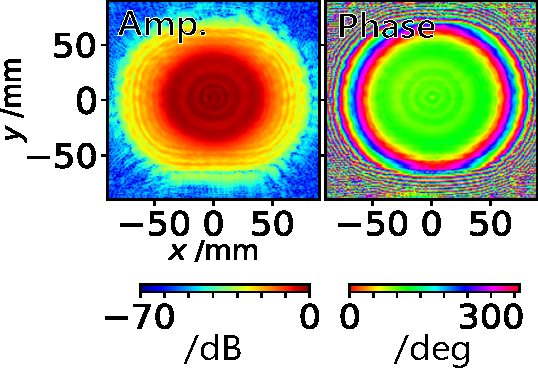
\includegraphics[width=0.9\linewidth]{Figures/NF_f1_Vpol.pdf}
\caption{%
Amplitude and phase maps measured near the aperture at 180~GHz. The feed horn is placed at Position A.
}
\label{fig:NF_f1_Vpol}
\end{figure}
%
%%%
%
\subsection{Comparison with Simulation}
%
\red{Pls move this paragraph to a section of LFT scaled model. \\
Former studies \cite{Kashima2018, Imada2018} had predicted that some far-sidelobe components would be created due to stray light, such as direct rays from the sky to the focal plane and three-time reflected rays. These sidelobes are designed to be reduced by the hood attached on the aperture (see Figure~\ref{fig:MeasSys}).}
\par
Figure~\ref{fig:Hood_F1_140G_map} shows the beam patterns at 140~GHz measured without and with the hood, and their $\theta_y = 0$ and $\theta_x = 0$ cuts are shown in Figure~\ref{fig:Hood_F1_140G_cut}. For without-hood case, sidelobe components caused by stray light are observed at $\theta_y \sim -50^\circ$ and $\theta_y \sim 40^\circ$, which correspond to direct rays and three-time reflected rays, respectively. These far-sidelobe features are reduced by around 20~dB when measured with the hood.
\par
Figure~\ref{fig:Hood_F1_140G_calc} shows the calculated beam pattern of the scaled LFT at 140~GHz without including the effects of the stray light. Its $\theta_y = 0$ and $\theta_x = 0$ cuts are also shown in Figure~\ref{fig:Hood_F1_140G_cut}. The measured beam pattern agrees with the calculated beam pattern at down to -50~dB level. 
%
\begin{figure}[!t]
\centering
\subfloat[Measured beam patterns without and with Hood at 140 GHz  ]{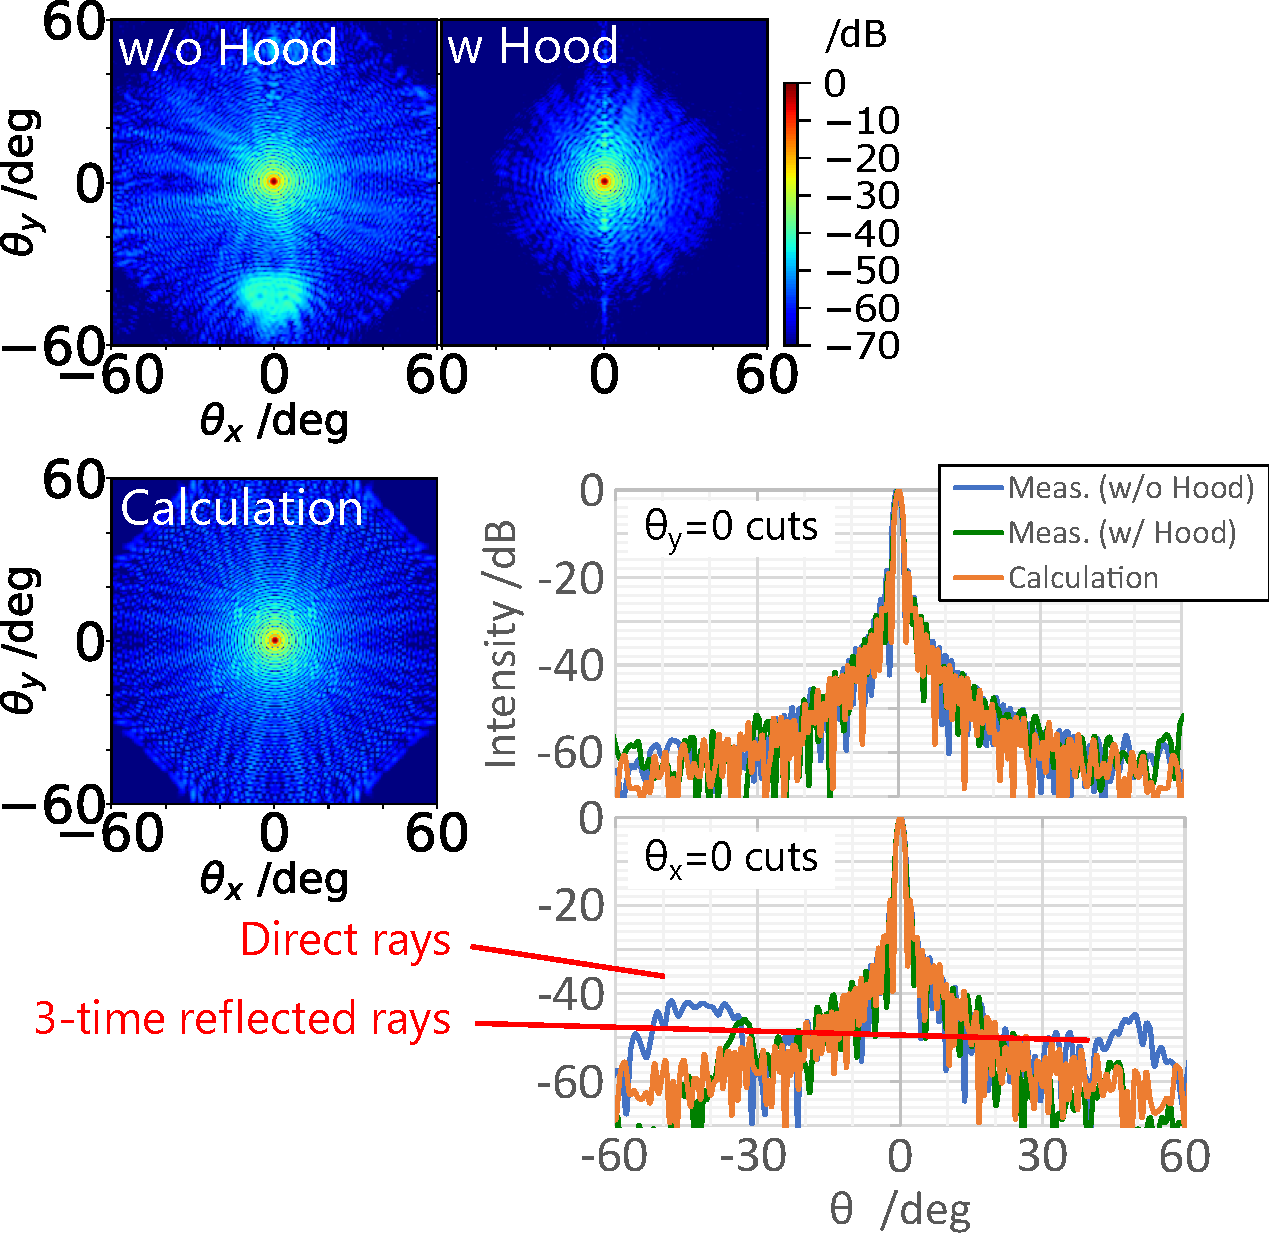
\includegraphics[width=0.9\linewidth]{Figures/Hood_F1_140G.pdf}%
\label{fig:Hood_F1_140G_map}}
\hfil
\subfloat[Calculated beam pattern at 140 GHz]{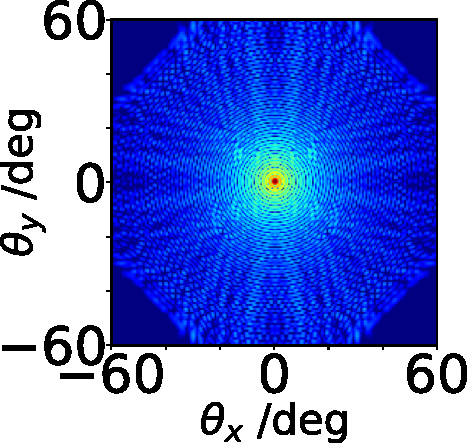
\includegraphics[width=0.5\linewidth]{Figures/Calc_F1_140G.pdf}%
\label{fig:Hood_F1_140G_calc}}
\hfil
\subfloat[$\theta_y = 0$ and $\theta_x = 0$ cuts]{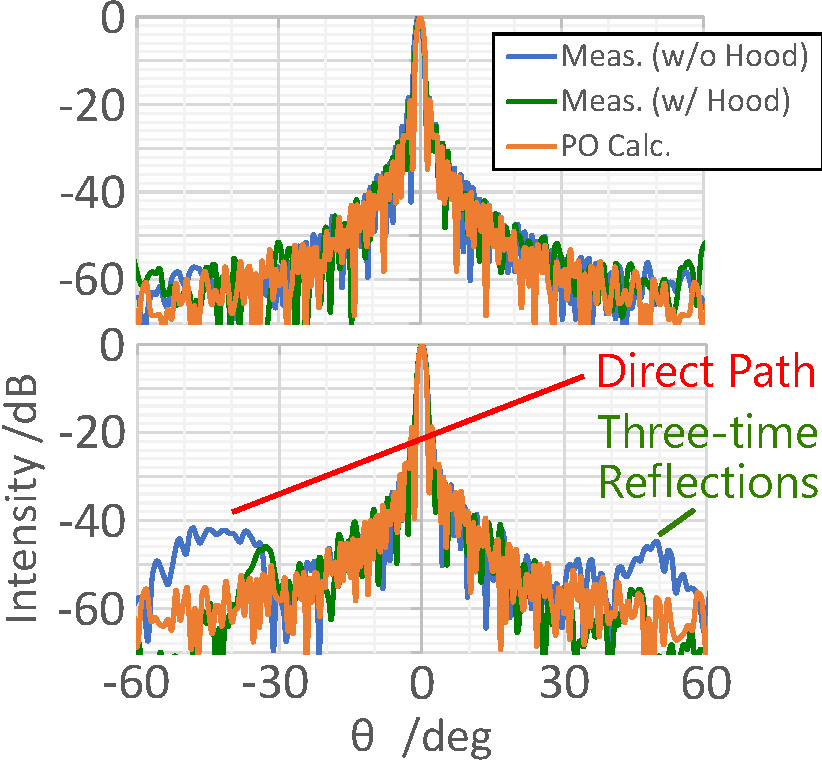
\includegraphics[width=0.8\linewidth]{Figures/Hood_F1_140G_cut.pdf}%
\label{fig:Hood_F1_140G_cut}}
\caption{%
\protect\subref{fig:Hood_F1_140G_map} The beam patterns at 140~GHz (corresponds to 35~GHz) measured without hood (\textit{left}) and with hood (\textit{right}). The feed horn was placed at Position A.
\protect\subref{fig:Hood_F1_140G_calc} A calculated beam pattern at 140~GHz for without-hood case. The calculation does not include the effects of stray light.
\protect\subref{fig:Hood_F1_140G_cut} Their $\theta_y = 0$ cuts (\textit{top}) and $\theta_x = 0$ cuts (\textit{bottom}). For without-hood case, sidelobe components caused by stray light are observed at $\theta_y \sim -50^\circ$ and $\theta_y \sim 40^\circ$, which correspond to direct rays from the sky to the focal plane and three-time reflected rays respectively. For with-hood case, these far-sidelobe features are drastically reduced; the measured beam pattern shows good agreement with the calculated beam pattern without stray light.
}
\label{fig:Hood_F1_140G}
\end{figure}
%
%%%
\subsection{Far-sidelobe Patterns}
%
Figure~\ref{fig:HVpol_140G} and Figure~\ref{fig:HVpol_220G} show the measured far-field beam patterns for each feed horn position of A, B and C at 140 GHz and 220 GHz respectively. The vertical structures at $\sim -50~\mathrm{dB}$ level were identified as near-field scanning noise caused by phase fluctuation during the measurement. The measurements have confirmed that the far-sidelobe components outside of $\sim \pm25^\circ$ are mostly suppressed down to -56~dB level except for some features caused by the remaining stray light. Also, beam patterns of two orthogonal polarization directions, V-pol and H-pol, are found to be consistent with each other at down to -40 dB level, even at the edges of the focal plane, namely feed horn positions of B and C.
%
\begin{figure*}[!t]
\centering
\subfloat[H-pol and V-pol beam patterns]{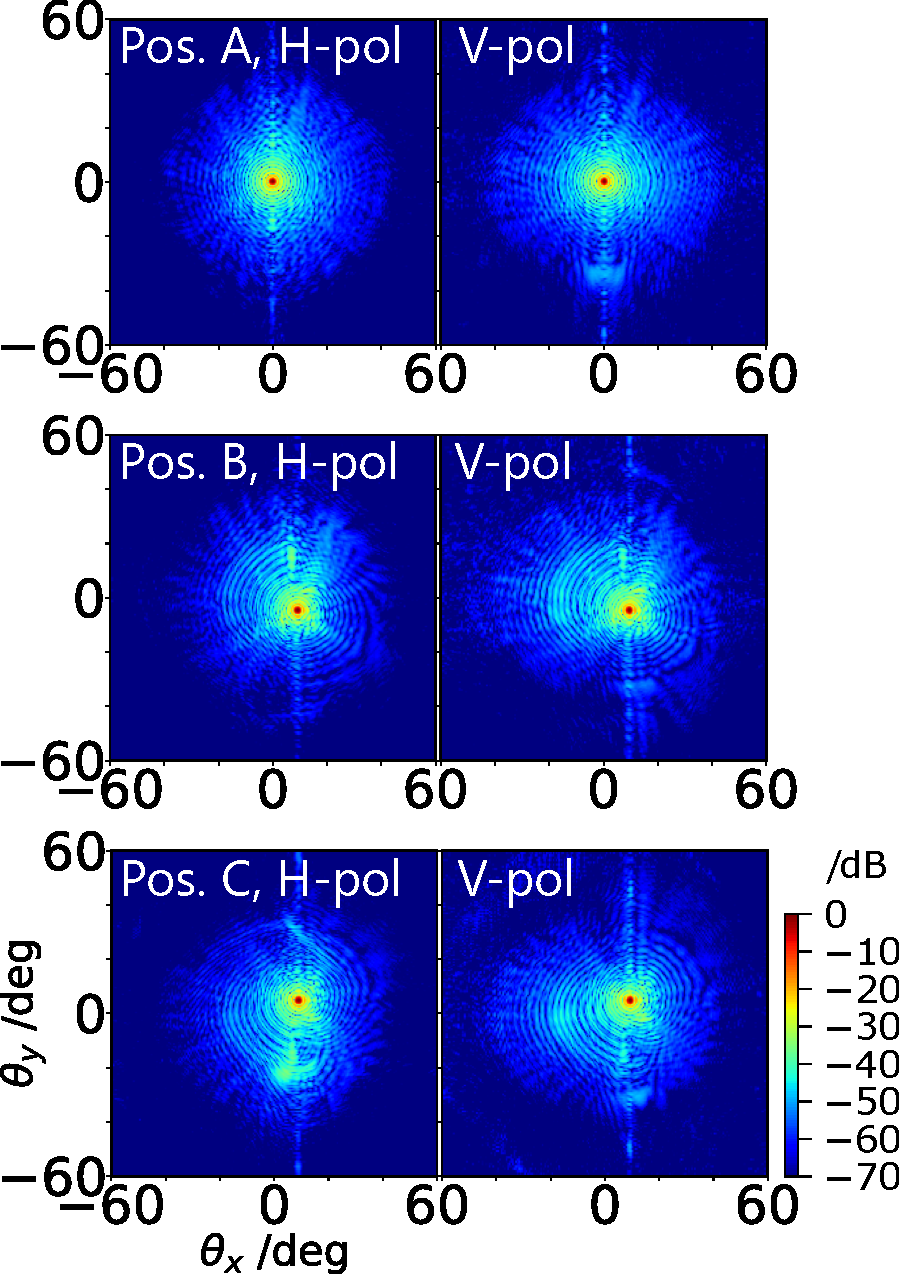
\includegraphics[width=0.5\linewidth]{Figures/HVpol_140G.pdf}%
\label{fig:HVpol_140G_map}}
\hfil
\subfloat[$\theta_x$ cuts of each beam pattern]{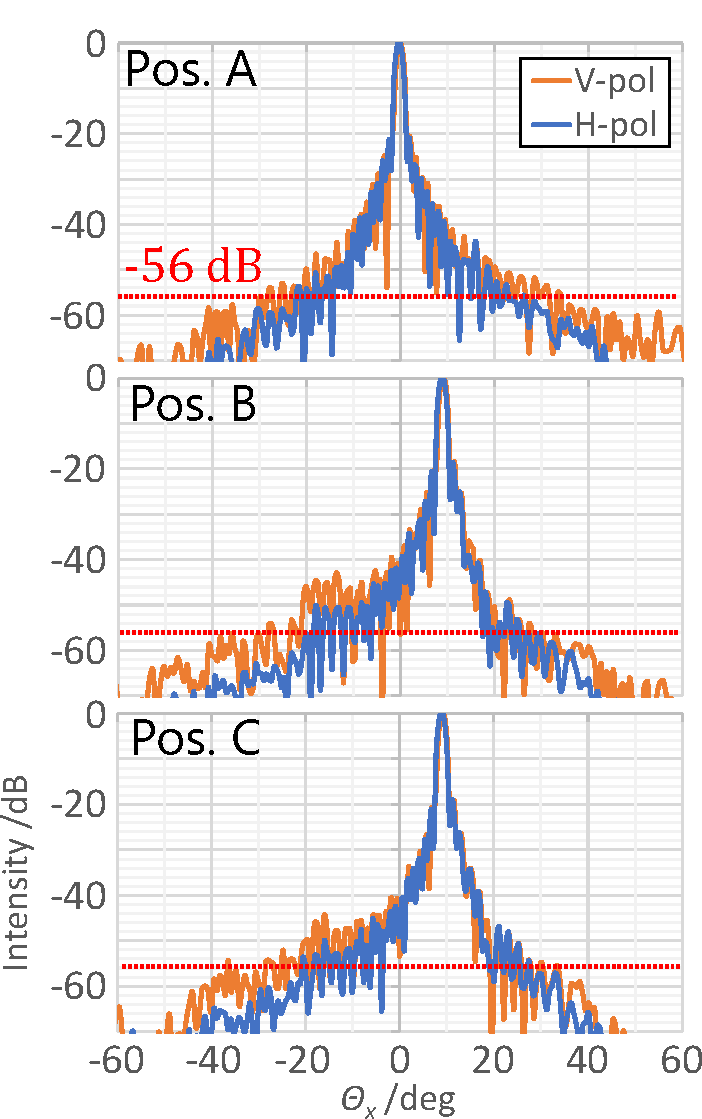
\includegraphics[width=0.4\linewidth]{Figures/HVpol_140G_Xcut}%
\label{fig:HVpol_140G_Xcut}}
\caption{%
\protect\subref{fig:HVpol_140G_map} H-pol and V-pol beam patterns at each feed horn position of A, B and C, measured at 140~GHz. \protect\subref{fig:HVpol_140G_Xcut} Their $\theta_y = 0$ cuts.
}
\label{fig:HVpol_140G}
\end{figure*}
%
\begin{figure*}[!t]
\centering
\subfloat[H-pol and V-pol beam patterns]{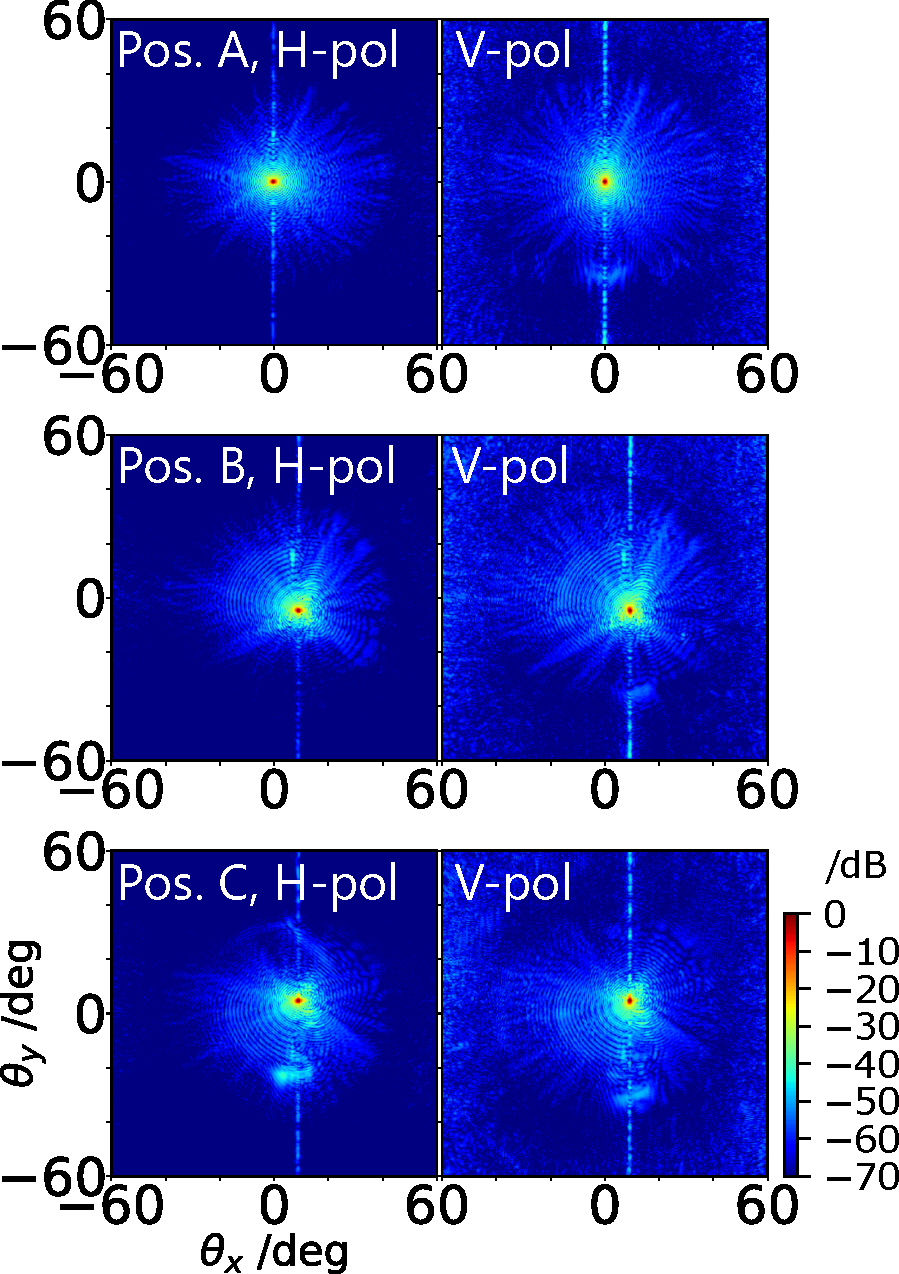
\includegraphics[width=0.5\linewidth]{Figures/HVpol_220G.pdf}%
\label{fig:HVpol_220G_map}}
\hfil
\subfloat[$\theta_x$ cuts of each beam pattern]{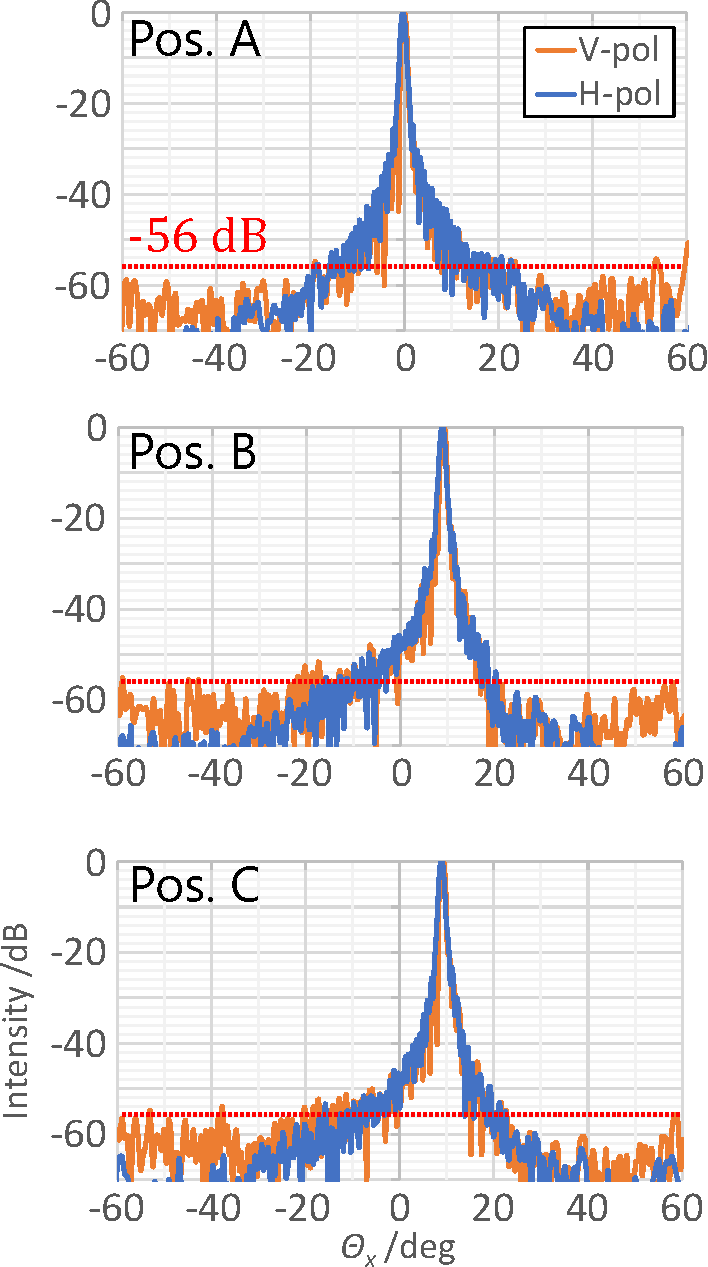
\includegraphics[width=0.4\linewidth]{Figures/HVpol_220G_Xcut}%
\label{fig:HVpol_220G_Xcut}}
\caption{%
\protect\subref{fig:HVpol_220G_map} H-pol and V-pol beam patterns at each feed horn position of A, B and C, measured at 220~GHz. \protect\subref{fig:HVpol_220G_Xcut} Their $\theta_y = 0$ cuts.
}
\label{fig:HVpol_220G}
\end{figure*}
%
%%%
\subsection{Cross Polarization pattern}
%
Figure~\ref{fig:HVpol_Xpol_180G_map} shows the measured cross-polarization patterns for feed horn positions of A, B and C at 180~GHz. The peak level of cross-polarization is less than -20 dB regardless of the feed horn position nor the polarization direction. The patterns show four peaks in diagonal directions, which are consistent with those of the feed horn shown in Figure~\ref{fig:FeedHornPattern}.
\par
%To evaluate the cross-polarization caused by the LFT mirrors themselves, we have also measured cross-polarization patterns with placing a free standing wire grid polarizer (Microtech Instruments G30x10-S) between the feed horn and the LFT scaled model. 
To evaluate cross polarization caused by the conical horn, a free-standing wire-grid (Microtech instruments G30x10-S) is placed in front of the conical horn, which reduces the cross polarization of the conical horn.
The results are shown in Figure~\ref{fig:HVpol_Xpol_180G_wiregrid} and \ref{fig:HVpol_Xpol_180G_cut}. 
From these results, we confirmed that the cross-polarization of the scaled LFT (\ref{fig:HVpol_Xpol_180G_map}) is caused mostly from the conical horn horn.
The cross-polarization created by the scaled LFT itself is verified to be less than -35~dB.
%
\begin{figure}[!t]
\centering
\subfloat[H-pol and V-pol cross-polarization patterns]{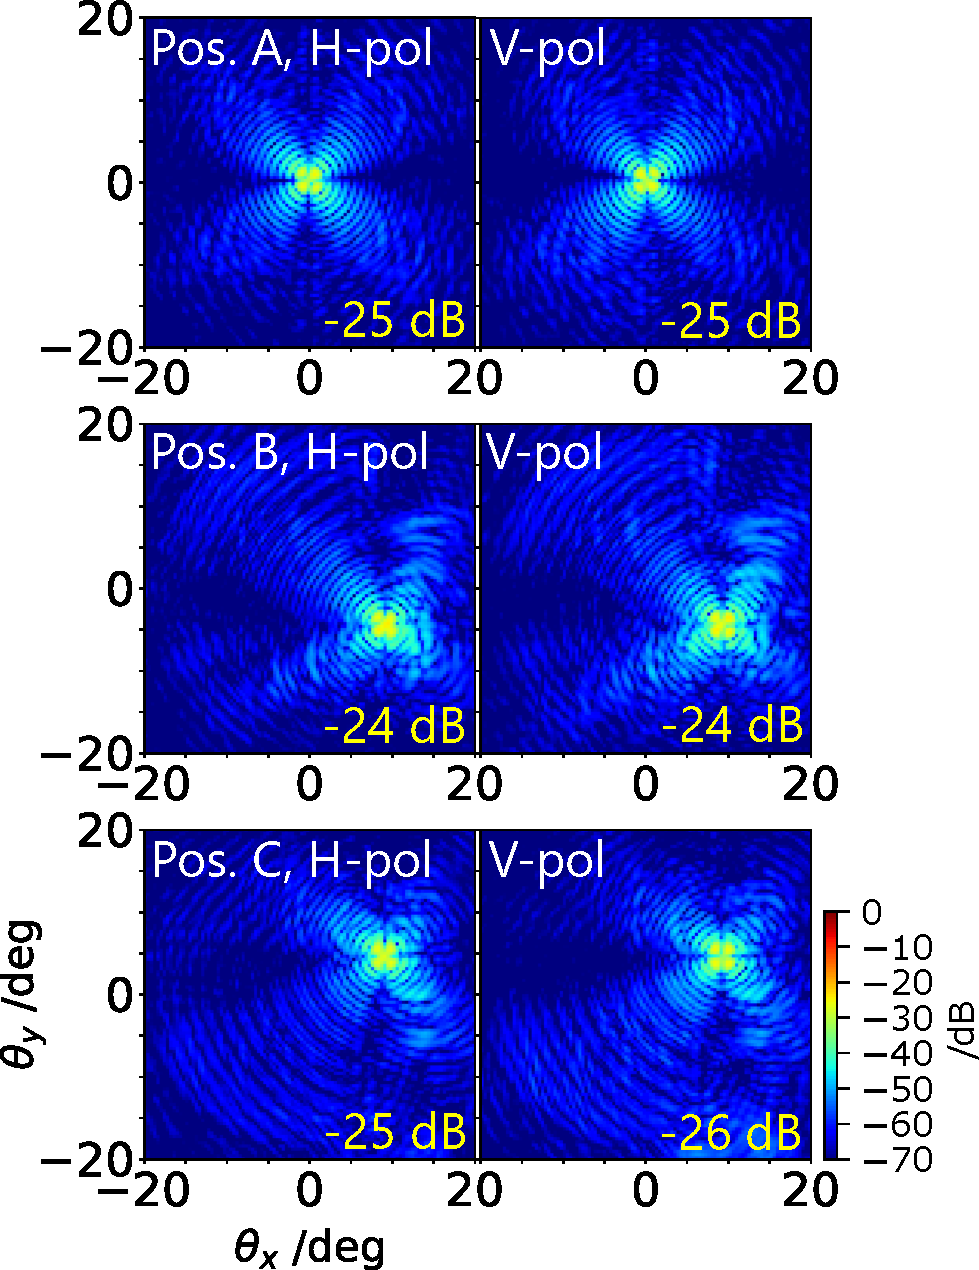
\includegraphics[width=\linewidth]{Figures/HVpol_Xpol_180G.pdf}%
\label{fig:HVpol_Xpol_180G_map}}
\hfil
\subfloat[V-pol cross-polarization pattern with wire grid]{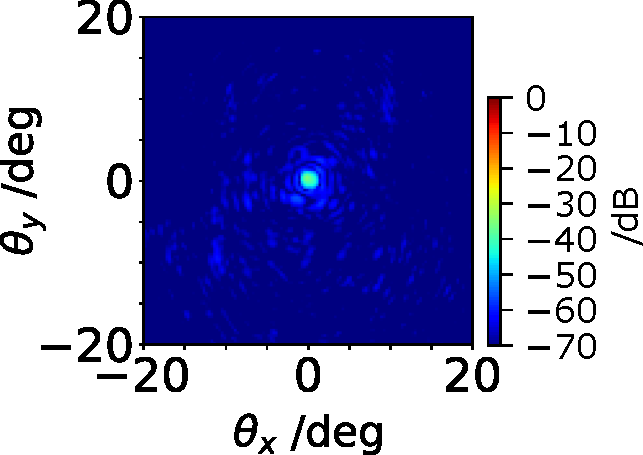
\includegraphics[width=0.7\linewidth]{Figures/HVpol_Xpol_180G_wiregrid.pdf}%
\label{fig:HVpol_Xpol_180G_wiregrid}}
\hfil
\subfloat[Cuts of V-pol patterns]{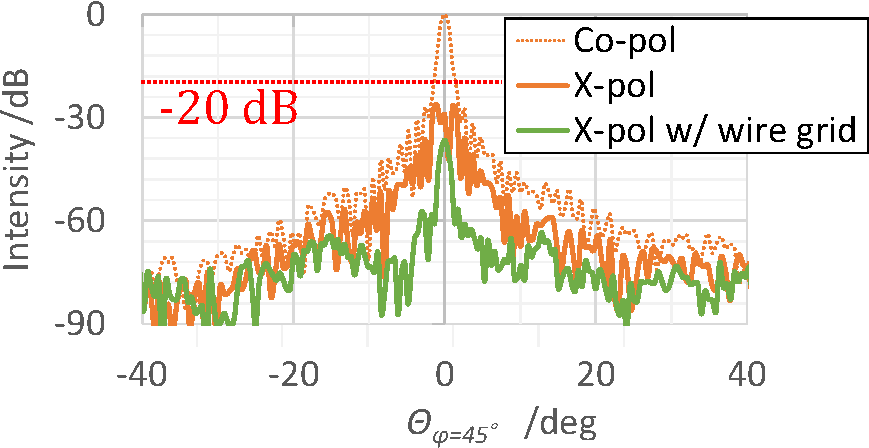
\includegraphics[width=0.9\linewidth]{Figures/HVpol_Xpol_180G_cut.pdf}%
\label{fig:HVpol_Xpol_180G_cut}}
\caption{%
\protect\subref{fig:HVpol_Xpol_180G_map} Cross-polarization beam patterns for H-pol and V-pol at each feed horn position of A, B and C, measured at 180~GHz. The values show the peak level of the cross-polarization.
\protect\subref{fig:HVpol_Xpol_180G_wiregrid} Cross-polarization beam pattern for V-pol at Position A, measured with a wire grid polarizer at 180~GHz. The peak level was -35~dB.
\protect\subref{fig:HVpol_Xpol_180G_cut} $\theta_y = 0$ cut of V-pol co-polarization pattern, and $\phi = 45^\circ$ cuts of V-pol cross-polarization patterns without and with wire grid polarizer.
}
\label{fig:HVpol_Xpol_180G}
\end{figure}
%
% (End of Results and Discussion)
%
\section{Summary}
We have developed a 1/4-scaled model of LiteBIRD LFT and its near-field beam measurement system to confirm the far-sidelobe patterns of LFT. We have measured beam patterns for two orthogonal polarization directions at the center and the edges of the focal plane. The measurement frequency was 140-220 GHz, which correspond to the lowest bands (35-55 GHz) of the full-scale LFT.
\par
The measurements are consistent with the simulated far-sidelobe patterns at -50~dB level, and have confirmed that some sidelobe features are due to stray light and are drastically reduced by the hood. Other far-sidelobe components were mostly less than -56 dB. We have also found that beams for two orthogonal polarization directions are consistent with each other down to -40~dB level. The cross-polarization level was also measured to be less than -20 dB, most of which is originated from the cross-polarization of the feed horn.
%
% (End of Summary)
%
%
% An example of a floating figure using the graphicx package.
% Note that \label must occur AFTER (or within) \caption.
% For figures, \caption should occur after the \includegraphics.
% Note that IEEEtran v1.7 and later has special internal code that
% is designed to preserve the operation of \label within \caption
% even when the captionsoff option is in effect. However, because
% of issues like this, it may be the safest practice to put all your
% \label just after \caption rather than within \caption{}.
%
% Reminder: the "draftcls" or "draftclsnofoot", not "draft", class
% option should be used if it is desired that the figures are to be
% displayed while in draft mode.
%
%\begin{figure}[!t]
%\centering
%\includegraphics[width=2.5in]{myfigure}
% where an .eps filename suffix will be assumed under latex, 
% and a .pdf suffix will be assumed for pdflatex; or what has been declared
% via \DeclareGraphicsExtensions.
%\caption{Simulation results for the network.}
%\label{fig_sim}
%\end{figure}
%
% Note that the IEEE typically puts floats only at the top, even when this
% results in a large percentage of a column being occupied by floats.
%
% An example of a double column floating figure using two subfigures.
% (The subfig.sty package must be loaded for this to work.)
% The subfigure \label commands are set within each subfloat command,
% and the \label for the overall figure must come after \caption.
% \hfil is used as a separator to get equal spacing.
% Watch out that the combined width of all the subfigures on a 
% line do not exceed the text width or a line break will occur.
%
%\begin{figure*}[!t]
%\centering
%\subfloat[Case I]{\includegraphics[width=2.5in]{box}%
%\label{fig_first_case}}
%\hfil
%\subfloat[Case II]{\includegraphics[width=2.5in]{box}%
%\label{fig_second_case}}
%\caption{Simulation results for the network.}
%\label{fig_sim}
%\end{figure*}
%
% Note that often IEEE papers with subfigures do not employ subfigure
% captions (using the optional argument to \subfloat[]), but instead will
% reference/describe all of them (a), (b), etc., within the main caption.
% Be aware that for subfig.sty to generate the (a), (b), etc., subfigure
% labels, the optional argument to \subfloat must be present. If a
% subcaption is not desired, just leave its contents blank,
% e.g., \subfloat[].
%
% An example of a floating table. Note that, for IEEE style tables, the
% \caption command should come BEFORE the table and, given that table
% captions serve much like titles, are usually capitalized except for words
% such as a, an, and, as, at, but, by, for, in, nor, of, on, or, the, to
% and up, which are usually not capitalized unless they are the first or
% last word of the caption. Table text will default to \footnotesize as
% the IEEE normally uses this smaller font for tables.
% The \label must come after \caption as always.
%
%\begin{table}[!t]
%% increase table row spacing, adjust to taste
%\renewcommand{\arraystretch}{1.3}
% if using array.sty, it might be a good idea to tweak the value of
% \extrarowheight as needed to properly center the text within the cells
%\caption{An Example of a Table}
%\label{table_example}
%\centering
%% Some packages, such as MDW tools, offer better commands for making tables
%% than the plain LaTeX2e tabular which is used here.
%\begin{tabular}{|c||c|}
%\hline
%One & Two\\
%\hline
%Three & Four\\
%\hline
%\end{tabular}
%\end{table}
%
% Note that the IEEE does not put floats in the very first column
% - or typically anywhere on the first page for that matter. Also,
% in-text middle ("here") positioning is typically not used, but it
% is allowed and encouraged for Computer Society conferences (but
% not Computer Society journals). Most IEEE journals/conferences use
% top floats exclusively. 
% Note that, LaTeX2e, unlike IEEE journals/conferences, places
% footnotes above bottom floats. This can be corrected via the
% \fnbelowfloat command of the stfloats package.
%

%
% if have a single appendix:
%\appendix[Proof of the Zonklar Equations]
% or
%\appendix  % for no appendix heading
% do not use \section anymore after \appendix, only \section*
% is possibly needed
%
% use appendices with more than one appendix
% then use \section to start each appendix
% you must declare a \section before using any
% \subsection or using \label (\appendices by itself
% starts a section numbered zero.)
%
%
% \appendices
% \section{Proof of the First Zonklar Equation}
% Appendix one text goes here.
%
% you can choose not to have a title for an appendix
% if you want by leaving the argument blank
% \section{}
% Appendix two text goes here.
%
%
% use section* for acknowledgment
\section*{Acknowledgment}
%
The authors would like to acknowledge Tetsuya Ito, Yoshinori Uzawa (NAOJ) and Tom Nitta (Univ. of Tsukuba) for 
their kind advice on design of near-field beam measurement system. We also would like to thank LiteBIRD Pre-phase A2 members for their many pieces of advice and discussion.
\par
This work was supported by 
the acceleration program of JAXA research and development directorate,
NAOJ support program, and
JSPS/MEXT KAKENHI Grant Numbers JP17H01115, JP15H05891, JP15H05743.
%The measurement is supported by an acceleration program of JAXA research and development directorate.
%
% Can use something like this to put references on a page
% by themselves when using endfloat and the captionsoff option.
\ifCLASSOPTIONcaptionsoff
  \newpage
\fi
%
% trigger a \newpage just before the given reference
% number - used to balance the columns on the last page
% adjust value as needed - may need to be readjusted if
% the document is modified later
%\IEEEtriggeratref{8}
% The "triggered" command can be changed if desired:
%\IEEEtriggercmd{\enlargethispage{-5in}}
%
% references section
%
% can use a bibliography generated by BibTeX as a .bbl file
% BibTeX documentation can be easily obtained at:
% http://mirror.ctan.org/biblio/bibtex/contrib/doc/
% The IEEEtran BibTeX style support page is at:
% http://www.michaelshell.org/tex/ieeetran/bibtex/
\bibliographystyle{IEEEtran}
% argument is your BibTeX string definitions and bibliography database(s)
\bibliography{ISSTT_Proceedings.bib}
%
%
% biography section
% 
% If you have an EPS/PDF photo (graphicx package needed) extra braces are
% needed around the contents of the optional argument to biography to prevent
% the LaTeX parser from getting confused when it sees the complicated
% \includegraphics command within an optional argument. (You could create
% your own custom macro containing the \includegraphics command to make things
% simpler here.)
%\begin{IEEEbiography}[{\includegraphics[width=1in,height=1.25in,clip,keepaspectratio]{mshell}}]{Michael Shell}
% or if you just want to reserve a space for a photo:
%
\begin{IEEEbiography}{Hayato Takakura}
Biography text here.
\end{IEEEbiography}
%
% if you will not have a photo at all:
%
\begin{IEEEbiographynophoto}{Yutaro Sekimoto}
received the Ph.D. degree from School of Science, University of Tokyo, Japan in 1994. 
He has been with ISAS/JAXA since 2017.
His research interests cover CMB B-mode polarization observations and millimeter-wave instrumentation.
\end{IEEEbiographynophoto}
%
\begin{IEEEbiographynophoto}{Junji Inatani}
Biography text here.
\end{IEEEbiographynophoto}
%
\begin{IEEEbiographynophoto}{Shingo Kashima}
Biography text here.
\end{IEEEbiographynophoto}
%
\begin{IEEEbiographynophoto}{Hiroaki Imada}
Biography text here.
\end{IEEEbiographynophoto}
%
\begin{IEEEbiographynophoto}{Takashi Hasebe}
Biography text here.
\end{IEEEbiographynophoto}
%%
\begin{IEEEbiographynophoto}{Toru Kaga}
Biography text here.
\end{IEEEbiographynophoto}
%
\begin{IEEEbiographynophoto}{Yoichi Takeda}
Biography text here.
\end{IEEEbiographynophoto}
%
%
\begin{IEEEbiographynophoto}{Norio Okada}
Biography text here.
\end{IEEEbiographynophoto}
% You can push biographies down or up by placing
% a \vfill before or after them. The appropriate
% use of \vfill depends on what kind of text is
% on the last page and whether or not the columns
% are being equalized.
%
%\vfill
%
% Can be used to pull up biographies so that the bottom of the last one
% is flush with the other column.
%\enlargethispage{-5in}
%
\end{document}